\section{Methodology}\label{method}
%Remove the weekly trend of the data to analyze the detailed changes that convey the device behavior at small time scales.

Our initial approach examined simple correlation analysis on sensor traces.  However, we quickly
found that correlation overly sensitive to fluctuations in the data.  {\bf Figure~\ref{fig:blah} shows
the sensitivity in the analysis using only correlation.}
Fundamentally, observed readings are driven by overlapping external phenomena.  Therefore,
if  sensors overlap spatio-temporally, their readings should be correlated.  What we observe in the data
is that the main driver for the readings of many of the sensors is outside temperature and weather.  It causes 
the heaters to turn on/off, the lights to turn on/off, occupancy to vary.  There were other factors, such as 
holiday scheduling and deadlines for student projects.  This made the sensor traces look correlated in
their raw feed.  In order to find unique relationships we needed to remove the common trends.

\subsection{Empirical Mode Decomposition}
Empirical Mode Decomposition (EMD) \cite{huang:emd1998} is a new techniques used for de-trending data.
Specifically, EMD detrends non-stationary, non-linear timeseries data.  A trend is defined as 
an intrinsically determined monotonic function within a certain temporal span or a function in which there 
can be at most one extremum within that temporal span.  A non-stationary signal is a signal whose mean and
variance change over time.  EMD is a process, rather than a theoretical tool.

We describe the process as follow:  for a signal \emph{X(t)}, let $m_1$ be the mean of its upper and
lower envelopes as determined from a cubic-spline interpolation of local maxima and minima. The locality 
is determined by an arbitrary parameter.

\begin{enumerate}
\item The first component $h_1$ is computed: $h_1=X(t)-m_1$
\item In the second sifting process, $h_1$ is treated as the data, and $m_{11}$ is the mean of $h_1$'s upper and lower envelopes: $h_{11}=h_1-m_{11}$
\item The procedure is repeated $k$ times, until $h_{1k}$ is a function: $h_{1(k-1)}-m_{1k}=h_{1k}$
\item Then it is designated as $c_1=h_{1k}$, the first functional component from the data, which contains the shortest period component of the signal. We separate it from the rest of the data: $X(t)-c_1 = r_1$, and the procedure is
repeated on $r_j: r_1-c_2 = r_2,\dots,r_{n-1} - c_n = r_n$
\end{enumerate}

The result is a set of functions called intrinsic mode functions (IMF); the number of functions in 
the set depends on the original signal~\cite{emd_process}.  An IMF is any 
function with the same number of extrema and zero crossings, with its envelopes being symmetric with respect to zero.
We run our correlation analysis on the shared IMF outputs between a pairs of signals.  In order to ensure 
that the IMFs corresponding to two distinct signals are on the same time scale, we use 
bivariate EMD \cite{rilling:biemd2007} to decompose two signals at once. The main use of EMD is for removing dominant trends to conduct a meaningful spectral analysis of the data.

\begin{figure*}
 \subfigure[EHP vs. Light]{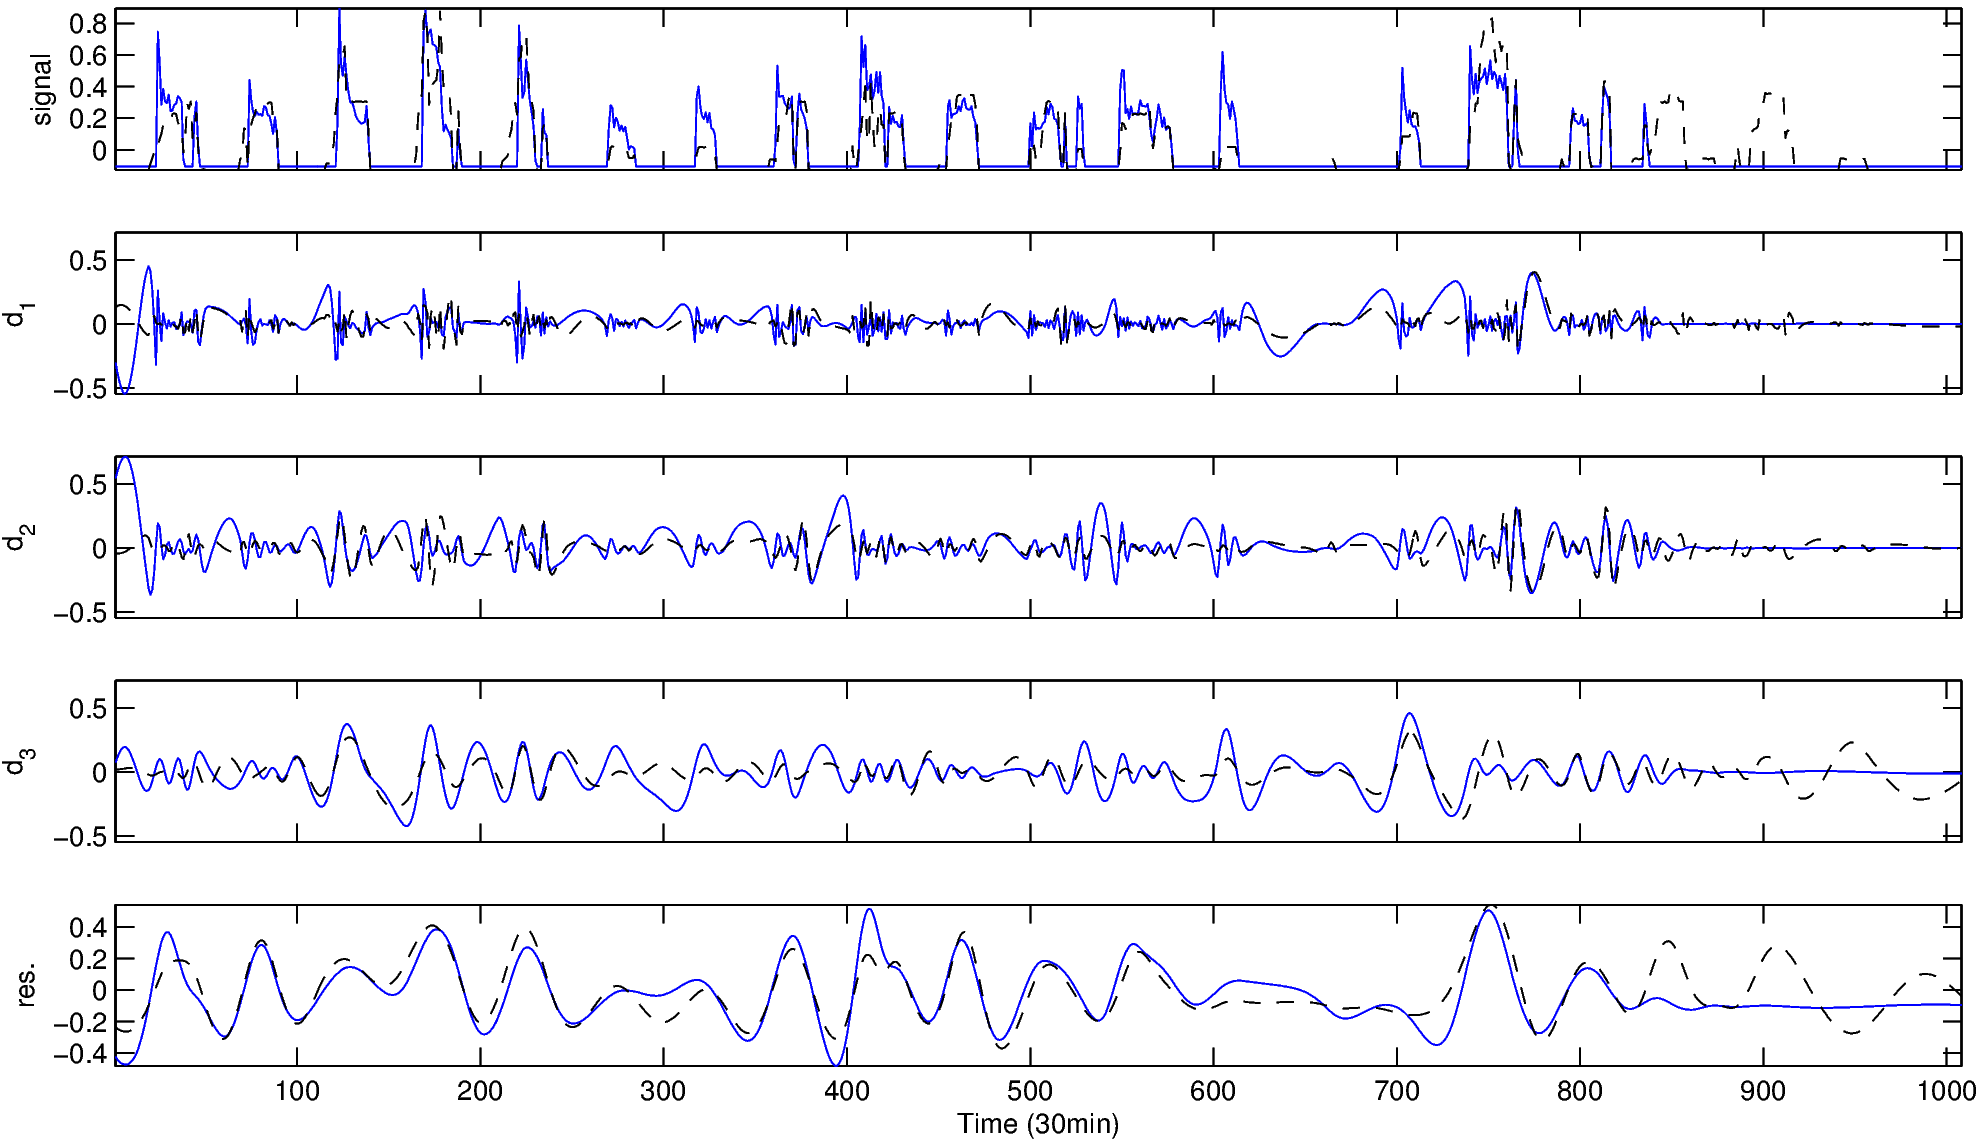
\includegraphics[width=\textwidth]{img/emd_25_26}}
 \subfigure[EHP vs. GHP]{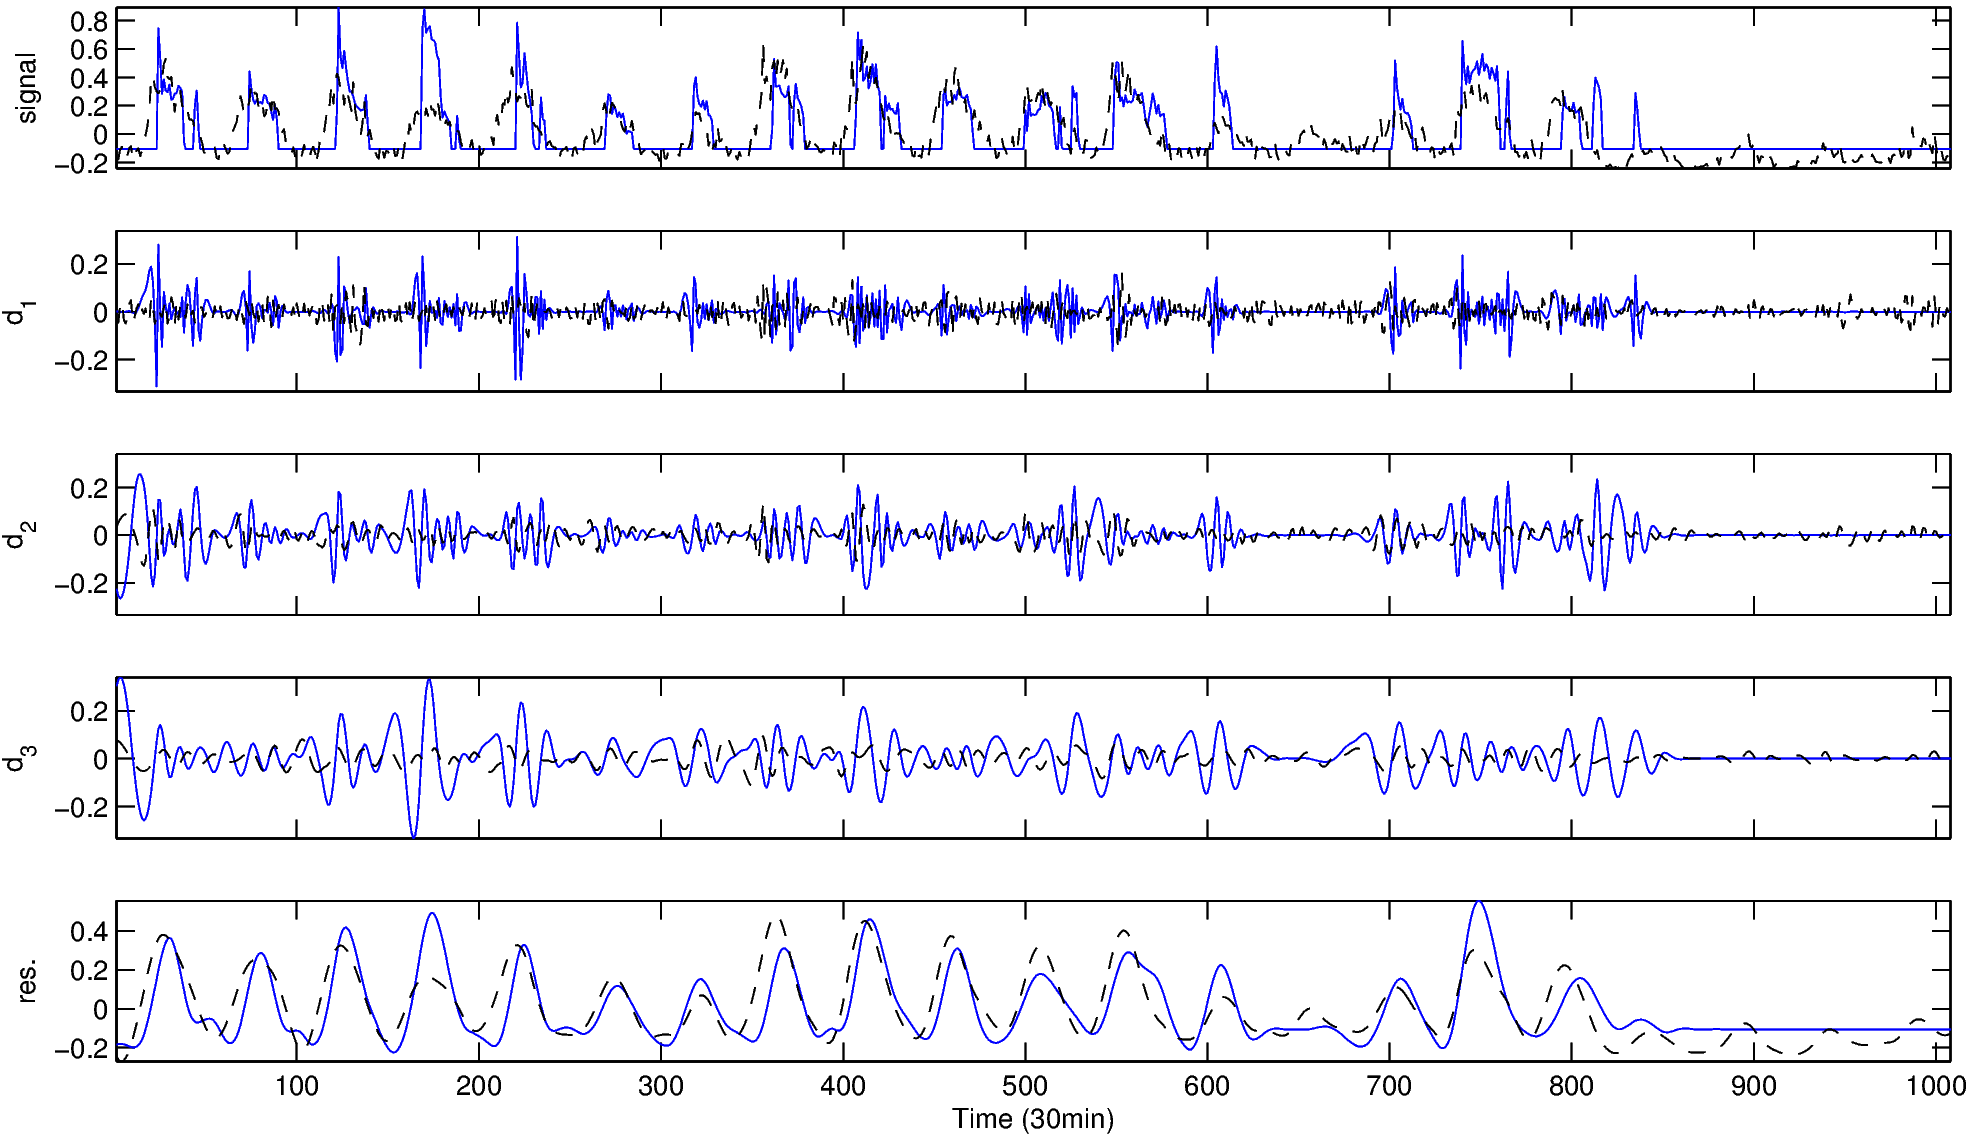
\includegraphics[width=\textwidth]{img/emd_25_41}}
 \caption{Empirical Mode Decomposition}
 %\label{fig:raw}
\end{figure*}
